\usetikzlibrary{calc}
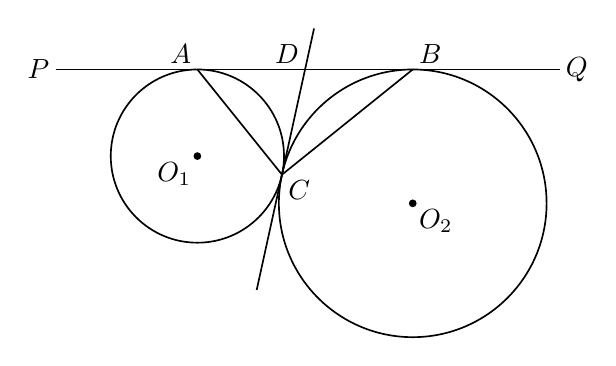
\begin{tikzpicture}[x=1cm,y=1cm,line width=.6pt,font=\normalsize]
\coordinate (O1) at (0,-1.1);
\coordinate (O2) at (2.73496,-1.7);
\coordinate (A) at (0,0);
\coordinate (B) at (2.73496,0);
\coordinate (C) at (1.07445,-1.33571);
\coordinate (D) at (1.36748,0);
\coordinate (P) at (-1.8,0);
\coordinate (Q) at (4.6,0);
\coordinate (Ttop) at (1.48159,0.52017);
\coordinate (Tbot) at (0.75302,-2.80088);
\draw (P)--(Q);
\draw (O1) circle[radius=1.1cm];
\draw (O2) circle[radius=1.7cm];
\draw (A)--(C);
\draw (B)--(C);
\draw (Ttop)--(Tbot);
\node[left=2pt,inner sep=0pt] at (P) {$P$};
\node[right=2pt,inner sep=0pt] at (Q) {$Q$};
\node[above left=2pt,inner sep=0pt] at (A) {$A$};
\node[above right=2pt,inner sep=0pt] at (B) {$B$};
\node[below right=2pt,inner sep=0pt] at (C) {$C$};
\node[above left=2pt,inner sep=0pt] at (D) {$D$};
\node[below left=2pt,inner sep=0pt] at (O1) {$O_{1}$};
\node[below right=2pt,inner sep=0pt] at (O2) {$O_{2}$};

% Explicit named circle-center points, painted after all region fills.
\fill (O1) circle[radius=1.4pt];
\fill (O2) circle[radius=1.4pt];
\end{tikzpicture}
